\documentclass[12pt]{article}
\usepackage{sbc-template}
\usepackage[T1]{fontenc}
\usepackage[utf8]{inputenc}
\usepackage[brazil]{babel}
\usepackage[hidelinks]{hyperref}
\usepackage{indentfirst,graphicx,url,booktabs,array,amsmath,flafter}
\sloppy
\title{Detecção de anomalias em transações Ethereum:\\avaliação temporal de Autoencoder e Isolation Forest}
\author{Marcelo Corni Alves\inst{1}, Saulo Moraes Villela\inst{1},\\
Heder Soares Bernardino\inst{1}, Alex Borges Vieira\inst{1}}
\address{Programa de Pós-Graduação em Ciência da Computação (PPGCC)\\
Universidade Federal de Juiz de Fora (UFJF) -- Juiz de Fora, MG, Brasil
\email{marcelo.corni@estudante.ufjf.br, saulo.moraes@ufjf.br}
\email{heder.bernardino@ufjf.br, alex.borges@ufjf.br}}
\begin{document}
\maketitle

\begin{abstract}
We compare Autoencoder and Isolation Forest on 523.9 million Ethereum transactions using 21 on-chain features and thresholds calibrated in June. At Q99.5, during July--November, they flag 761,411 and 728,748 MEV-associated transactions, sharing 413,944. Among all transactions flagged by both models, 40.42\% are MEV-associated. Their union recovers 1,076,215 associated transactions. In December's stress window, Autoencoder flags 250,565 associated transactions versus 18,434 for Isolation Forest. These findings inform investigation priorities across temporal regimes. Future work will adapt structural front-running detection algorithms and semantically validate candidate patterns.
\end{abstract}

\begin{resumo}
Comparamos Autoencoder e Isolation Forest em 523,9 milhões de transações Ethereum, com 21 atributos on-chain e limiares calibrados em junho. Em Q99,5, de julho a novembro, sinalizam 761.411 e 728.748 transações associadas a bots MEV, compartilhando 413.944. Entre todas as transações sinalizadas por ambos, 40,42\% são associadas a MEV. A união recupera 1.076.215 associadas. No estresse de dezembro, o Autoencoder sinaliza 250.565 associadas, contra 18.434 do Isolation Forest. Os achados orientam prioridades de investigação em diferentes regimes temporais. Como continuidade, propomos adaptar algoritmos estruturais de detecção de front-running e validar semanticamente os padrões candidatos.
\end{resumo}

\section{Introdução}
A atividade transacional da Ethereum reúne transferências, contratos inteligentes e operações automatizadas com comportamentos heterogêneos. Identificar desvios permite priorizar investigações e caracterizar atividades relacionadas ao \textit{Maximal Extractable Value} (MEV). Nessa perspectiva, escores de anomalia e evidências estruturais de \textit{front-running} oferecem perspectivas distintas sobre o comportamento transacional \cite{Torres2021}.

Comparamos Autoencoder (AE) e Isolation Forest (IF) em todos os registros disponíveis de 2025 na fonte utilizada, sem amostragem de blocos nem indicadores de mercado ou sentimento. Investigamos como a sinalização evolui sob limiares congelados, quanto os conjuntos concordam e como os escores ordenam transações associadas a endereços históricos de bots MEV. As contribuições são uma avaliação temporal em 523.937.952 transações, a quantificação das sinalizações compartilhadas e exclusivas, e a comparação da recuperação de transações associadas a bots MEV nos diferentes recortes.

\section{Fundamentação e trabalhos relacionados}
Sakurada e Yairi \cite{Sakurada2014} empregam autoencoders para detectar anomalias por reconstrução não linear. Liu et al.\ \cite{Liu2008} propõem o isolamento como princípio de detecção. É necessário distinguir qualidade da ordenação e concentração na cauda extrema dos escores.

Na Ethereum, Farrugia et al.\ \cite{Farrugia2020} estudam contas ilícitas por classificação supervisionada de propriedades de contas e de suas transações. Torres et al.\ \cite{Torres2021} identificam padrões estruturais de inserção, deslocamento e supressão em \textit{front-running}. Neste trabalho, a unidade analisada é a transação, os modelos são ajustados sem rótulos e o Label Cloud fornece uma referência externa após a inferência. Essa organização permite examinar a relação entre anormalidade transacional, associação a bots MEV e mudanças temporais.

A literatura de adaptação a \textit{concept drift} discute mudanças na relação entre entradas e alvos \cite{Gama2014}. Aqui, caracterizamos mudanças marginais dos atributos e dos escores. Na avaliação auxiliar desbalanceada, ROC-AUC, \textit{Average Precision} (AP) e concentração no topo do ranking descrevem aspectos complementares da ordenação \cite{Saito2015}.

\section{Metodologia}
\subsection{Dados e recortes temporais}
Utilizamos Parquets diários de transações da Ethereum Mainnet do AWS Public Blockchain Data \cite{AWSBlockchain}. Os 365 dias de 2025 totalizam 523.937.952 registros, processados integralmente em UTC, e 2.608.546 alturas de blocos observadas. A seleção abrange todos os registros disponíveis na fonte utilizada, com verificação da integridade dos arquivos e da consistência dos registros.

\begin{table}[htbp]
\centering\small
\caption{Recortes de 2025, datas inclusivas em UTC.}
\label{tab:recortes}
\begin{tabular}{@{}llrl@{}}
\toprule
Recorte & Período & Transações & Uso \\
\midrule
Treino & 01/01--30/04 & 147.512.905 & Ajuste \\
Pectra & 01/05--31/05 & 41.982.829 & Retrospectiva \\
Validação & 01/06--30/06 & 41.950.663 & Calibração \\
Teste & 01/07--30/11 & 241.020.375 & Avaliação \\
Fusaka/BPO1 & 01/12--09/12 & 14.264.473 & Transição \\
Estresse & 10/12--31/12 & 37.206.707 & Estresse temporal \\
\bottomrule
\end{tabular}
\end{table}

A Tabela~\ref{tab:recortes} separa ajuste, calibração e avaliação. Maio constitui uma análise retrospectiva, pois utiliza limiares estimados em junho. As transições abrangem Pectra, ativada em 7 de maio, e Fusaka/BPO1, em 3 e 9 de dezembro \cite{Pectra2025,Fusaka2025}. Esses marcos organizam a comparação dos regimes transacionais ao longo do ano.

\subsection{Representação e pré-processamento}
Cada transação é representada pelos 21 atributos da configuração B (Tabela~\ref{tab:atributos}). Contagens e ranks intrabloco utilizam todos os registros disponíveis do bloco. A representação caracteriza o comportamento da transação após sua inclusão e execução.

\begin{table}[htbp]
\centering\small
\caption{Atributos utilizados pelos modelos. $\ell(x)=\ln(1+x)$.}
\label{tab:atributos}
\begin{tabular}{@{}p{2.7cm}p{11.8cm}@{}}
\toprule
Grupo & Atributos \\
\midrule
Execução e valor & $\ell$(gás usado); gás usado/limite; $\ell$(valor); $\ell$(nonce); status do recibo. \\
Taxas & $\ell$(preço efetivo); $\ell$(taxa máxima); $\ell$(prioridade máxima); preço efetivo/taxa máxima. \\
Tipos & Indicadores dos tipos 0, 1 e 3. \\
Contexto do bloco & Posição relativa; $\ell$(número de transações); $\ell$(contagens por remetente e destinatário); rank percentual do preço efetivo. \\
Tempo & Seno/cosseno da hora e do dia da semana. \\
\bottomrule
\end{tabular}
\end{table}

Os nove atributos logarítmicos são normalizados por mediana e intervalo interquartil (IQR) estimados apenas no treino: $z=(\ell(x)-m_{\rm treino})/\mathrm{IQR}_{\rm treino}$. IQR nulo recebe escala unitária. Para taxas máximas e de prioridade, tipos legados 0/1 são excluídos do ajuste da escala e mantidos em zero. Indicadores, razões, ranks e componentes cíclicos preservam sua escala. Tipos 2 e 4 não possuem indicador próprio. Os dados são armazenados em precisão dupla e convertidos para \texttt{float32} na entrada dos modelos.

\subsection{Modelos, calibração e avaliação}
O AE possui arquitetura $21\!\to\!16\!\to\!8\!\to\!4\!\to\!8\!\to\!16\!\to\!21$, LeakyReLU com inclinação 0,1 e saída linear. O ajuste emprega AdamW, taxa $10^{-3}$, decaimento de pesos $10^{-5}$, lotes de 65.536 e precisão mista. A validação interna reserva transações com $\mathrm{row\_id}\bmod10=0$, sendo o identificador formado pelo número do bloco deslocado em 32 bits e pelo índice intrabloco. São 132.718.736 exemplos de ajuste e 14.794.169 de validação interna, no mesmo intervalo de treino. Essa reserva não substitui o teste temporal. Foram executadas 200 épocas; o modelo selecionado corresponde à menor perda interna, 0,1110, na época 197.

O IF utiliza 200 árvores, até 8.192 exemplos por árvore, todos os atributos e \texttt{contamination=auto}. O subconjunto de ajuste é determinístico: $h(\mathrm{row\_id})\bmod N<500.000$, para $N=147.512.905$. A regra selecionou 500.637 transações; esse subconjunto difere da amostragem interna de cada árvore. Ambos os modelos usam semente 42 e produzem escores para todos os registros. A comparação considera essas configurações de ajuste e sua aplicação à mesma população de avaliação.

O AE utiliza erro quadrático médio de reconstrução; o IF, o negativo de \texttt{score\_samples}. Escores maiores indicam maior anormalidade. Para cada método, estimamos em junho os quantis exatos Q99, Q99,5 e Q99,9 e sinalizamos $s(x)\geq\tau$. Os limiares ficam congelados nas demais janelas. Q99,5 é a referência principal, com $\tau_{AE}=0{,}40999$ e $\tau_{IF}=0{,}57341$. Empates podem afastar ligeiramente a taxa de calibração do valor nominal.

A concordância é $J(A,I)=|A\cap I|/|A\cup I|$. A mudança marginal é caracterizada por PSI, com intervalos definidos por decis do treino e piso $10^{-6}$, e distância de Kolmogorov--Smirnov aproximada sobre até 101 quantis do treino. Não são produzidos valores-$p$ nem inferências causais.

A referência auxiliar é um CSV histórico do Etherscan Label Cloud \cite{EtherscanLabels}, com 3.913 linhas e 3.750 endereços únicos. A associação positiva corresponde ao remetente constar como \texttt{mev\_bot}; as demais transações são denominadas não associadas. Trata-se de associação histórica de endereços, não de confirmação de ataques individuais. O snapshot possui data desconhecida e categorias reconstruídas a partir do arquivo histórico. Rótulos não participam do ajuste ou da calibração. ROC-AUC e AP utilizam todos os grupos de escores empatados; apenas as curvas são reduzidas para visualização. Avaliamos também \textit{precision}, \textit{recall} e concentração nos 1\% maiores escores, com desempate pelo identificador da transação.

\subsection{Reprodutibilidade}
O código está disponível no \href{https://github.com/marcelocorni/anomalias-ae-if-2025}{repositório público no GitHub}. O arquivo \texttt{uv.lock} fixa as dependências; o código e as configurações definem atributos, janelas, semente e hiperparâmetros. O comando \texttt{python scripts/executar\_etapa4.py --executar} integra processamento, avaliações e figuras. Manifestos registram hashes de entradas e saídas, contagens e tempos, com retomada de etapas conferidas. Os Parquets da AWS e o CSV histórico do Label Cloud são entradas externas, não versionadas; o CSV deve ser obtido separadamente e corresponde ao SHA-256 definido na configuração. A documentação descreve a preparação do ambiente e dos caminhos locais.

\section{Resultados e discussão}
\subsection{Sinalização e resposta temporal}
\begin{table}[htbp]
\centering\small
\caption{Sinalização em Q99,5. A interseção reúne todas as transações sinalizadas pelos dois modelos, associadas ou não a bots MEV.}
\label{tab:sinalizacao}
\begin{tabular}{@{}lrrrr@{}}
\toprule
Recorte & AE (\%) & IF (\%) & Interseção & Jaccard \\
\midrule
Treino & 0,858 & 0,411 & 163.048 & 0,095 \\
Pectra & 0,872 & 0,468 & 70.072 & 0,142 \\
Validação & 0,500 & 0,500 & 40.424 & 0,107 \\
Teste & 2,583 & 1,156 & 1.024.167 & 0,128 \\
Fusaka/BPO1 & 10,539 & 1,453 & 109.941 & 0,069 \\
Estresse & 17,385 & 2,667 & 523.147 & 0,075 \\
\bottomrule
\end{tabular}
\end{table}

A Tabela~\ref{tab:sinalizacao} mostra que manter o limiar não mantém o volume sinalizado. No teste de julho a novembro, o AE sinaliza 6.225.429 transações (2,583\%) e o IF, 2.787.088 (1,156\%). A interseção contém 1.024.167 registros e a união, 7.988.350: Jaccard de 0,128.

No estresse, o AE sinaliza 17,385\%, aproximadamente 34,8 vezes a taxa de calibração; o IF sinaliza 2,667\%, cerca de 5,3 vezes. O aumento também ocorre em Q99 e Q99,9. A expansão mais acentuada do AE evidencia maior sensibilidade ao regime transacional de dezembro, enquanto o IF preserva um conjunto sinalizado mais restrito.

O PSI do preço efetivo passa de 0,763 no teste para 2,958 no estresse, em relação ao treino; a distância KS aproximada passa de 0,307 para 0,701. Para a taxa máxima, o PSI passa de 0,452 para 1,606.

\subsection{Associação auxiliar e ordenação dos escores}
\begin{table}[htbp]
\centering\small
\caption{Transações associadas a bots MEV sinalizadas em Q99,5.}
\label{tab:mev-bot}
\begin{tabular}{@{}lrrrr@{}}
\toprule
Recorte & AE & IF & Interseção & União \\
\midrule
Treino & 6.249 & 8.097 & 3.074 & 11.272 \\
Pectra & 9.544 & 6.420 & 3.193 & 12.771 \\
Validação & 23.010 & 23.769 & 8.920 & 37.859 \\
Teste & 544.738 & 757.192 & 350.857 & 951.073 \\
Fusaka/BPO1 & 35.508 & 10.800 & 5.607 & 40.701 \\
Estresse & 75.354 & 13.313 & 5.014 & 83.653 \\
\bottomrule
\end{tabular}
\end{table}

A Tabela~\ref{tab:mev-bot} apresenta quantidades de transações, e não de endereços distintos. Em Q99,5 no teste, o AE recupera 761.411 transações associadas a \texttt{mev\_bot} e o IF, 728.748. A interseção contém 413.944 associadas, enquanto 347.467 são exclusivas do AE e 314.804, do IF. A união recupera 1.076.215 associadas, correspondentes a 24,02\% da população de referência do recorte.

\begin{figure}[htbp]
\centering
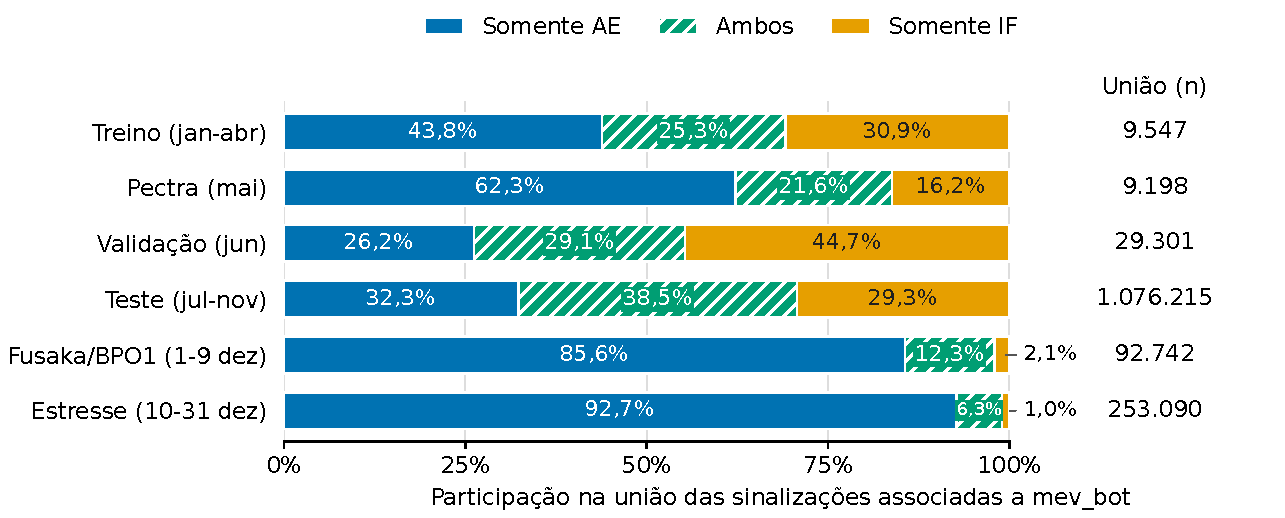
\includegraphics[width=\linewidth]{imagens/intersecoes-mev-q995.pdf}
\caption{Composição das transações associadas a \texttt{mev\_bot} sinalizadas em Q99,5. Cada barra representa 100\% da união dos modelos no recorte; a coluna à direita informa seu total de transações.}
\label{fig:intersecoes}
\end{figure}

A Figura~\ref{fig:intersecoes} evidencia a mudança na composição das sinalizações. No teste, 32,3\% da união são exclusivos do AE, 38,5\% são compartilhados e 29,3\% são exclusivos do IF. No estresse, a parcela exclusiva do AE alcança 92,7\%, enquanto a exclusiva do IF corresponde a 1,0\%.

As 413.944 associadas representam 40,42\% das 1.024.167 transações sinalizadas pelos dois modelos. Essa concentração supera os 12,23\% do conjunto do AE e os 26,15\% do IF. A interseção oferece, portanto, um conjunto menor e mais concentrado em associados no teste, enquanto a união amplia a recuperação. São alternativas quantitativas para organizar prioridades de investigação.

Na transição Fusaka/BPO1, os modelos compartilham 11.418 transações associadas e sua união reúne 92.742. No estresse, a interseção contém 15.909; 234.656 são exclusivas do AE e 2.525, do IF. A união recupera 253.090 associadas (77,62\%), frente às 250.565 do AE isolado. Assim, a contribuição exclusiva do IF à recuperação é mais expressiva no teste do que no estresse, evidenciando que os benefícios da união variam entre regimes temporais.

\begin{table}[htbp]
\centering\small
\caption{Ordenação dos escores frente à associação MEV. $P@1\%$ é a precision nos 1\% maiores escores; Prev. é a prevalência (\%).}
\label{tab:associacao}
\begin{tabular}{@{}lrrrrrrr@{}}
\toprule
 & & \multicolumn{2}{c}{ROC-AUC} & \multicolumn{2}{c}{AP} & \multicolumn{2}{c}{$P@1\%$ (\%)} \\ Recorte & Prev. & AE & IF & AE & IF & AE & IF \\
\midrule
Treino & 0,859 & 0,6432 & 0,9129 & 0,0128 & 0,0442 & 0,58 & 1,22 \\
Pectra & 1,028 & 0,7132 & 0,9210 & 0,0277 & 0,0633 & 4,29 & 4,12 \\
Validação & 1,273 & 0,8111 & 0,9421 & 0,1076 & 0,1219 & 19,87 & 15,79 \\
Teste & 1,859 & 0,7690 & 0,9481 & 0,0866 & 0,2067 & 8,17 & 29,26 \\
Fusaka/BPO1 & 1,010 & 0,6189 & 0,9040 & 0,0329 & 0,0524 & 8,85 & 5,67 \\
Estresse & 0,876 & 0,6309 & 0,8822 & 0,0286 & 0,0349 & 7,12 & 1,71 \\
\bottomrule
\end{tabular}
\end{table}

A Tabela~\ref{tab:associacao} evidencia dependência da janela e da métrica. No teste, a prevalência da associação histórica é 1,859\%. O IF apresenta ROC-AUC de 0,9364 e AP de 0,1741, superiores aos 0,6399 e 0,0738 do AE. Nos 1\% maiores escores, a proporção de associados é 26,32\% para IF e 14,35\% para AE: 14,16 e 7,72 vezes a prevalência, respectivamente.

\begin{figure}[htbp]
\centering
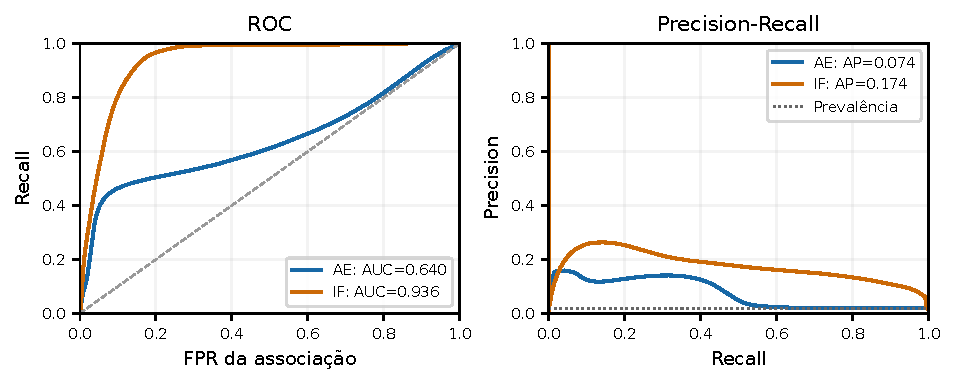
\includegraphics[width=\linewidth]{imagens/curvas-teste.pdf}
\caption{ROC e Precision-Recall no teste. A linha horizontal representa a prevalência da associação histórica. As métricas integram todos os grupos de escores.}
\label{fig:curvas}
\end{figure}

A Figura~\ref{fig:curvas} complementa as contagens de Q99,5 ao apresentar a ordenação dos escores em diferentes pontos de operação.

No estresse, AP do AE é 0,0595 e supera 0,0266 do IF, embora a ROC-AUC do IF ainda seja ligeiramente maior. Nos 1\% maiores escores, o AE concentra 9,42\% de associados; o IF, apenas 0,17\%, abaixo da prevalência de 0,876\%. O IF ordena grande parte dos associados acima dos não associados, mas coloca poucos na cauda extrema. Portanto, ROC-AUC elevada não garante boa priorização sob orçamento pequeno de investigação.

O \textit{recall} do AE em Q99,5 no estresse alcança 76,84\%, acompanhado por taxa de sinalização de 17,38\% e \textit{precision} auxiliar de 3,87\%. A leitura conjunta de contagens, \textit{precision}, \textit{recall} e AP permite comparar tanto a recuperação dos associados quanto a concentração obtida no conjunto priorizado.

\section{Conclusões e trabalhos futuros}
A análise de 523.937.952 transações mostra que Autoencoder e Isolation Forest oferecem respostas distintas às mudanças transacionais de 2025. No teste de julho a novembro, o IF combina maior AP com recuperação próxima à do AE: 728.748 e 761.411 transações associadas a bots MEV, respectivamente, sinalizando menos da metade do volume do AE. A interseção reúne 413.944 associadas entre 1.024.167 sinalizações compartilhadas, uma concentração de 40,42\%. A união amplia a recuperação para 1.076.215 associadas, incluindo contribuições exclusivas dos dois métodos.

No estresse de dezembro, o AE recupera 250.565 transações associadas, contra 18.434 do IF, e a união alcança 253.090. Os resultados distinguem políticas de priorização: selecionar a interseção concentra a associação MEV no teste, enquanto considerar a união amplia a cobertura, com contribuição adicional dependente do período. Essa comparação orienta a escolha de métodos e combinações conforme o regime transacional e o volume de investigação pretendido.

Como continuidade, propomos adaptar os algoritmos de Torres et al.\ \cite{Torres2021} ao contexto da Ethereum de 2025 para gerar candidatos a padrões de inserção, deslocamento e supressão. A geração estrutural será independente dos escores, permitindo comparar a cobertura do AE, do IF e de suas sinalizações compartilhadas e exclusivas sobre uma referência comum de eventos.

Esses candidatos serão submetidos a avaliação semântica, combinando ordem das transações, chamadas de contratos, recibos, logs, rastros de execução e fluxos de ativos. A análise examinará os papéis dos participantes e os efeitos econômicos das operações, com simulações de cenários alternativos de execução quando pertinentes. Essa etapa permitirá verificar se as estruturas encontradas correspondem efetivamente aos padrões investigados e medir como os modelos priorizam eventos validados. A integração entre detecção não supervisionada, regras estruturais e evidência semântica constitui o próximo passo para avançar da seleção de transações à avaliação de padrões concretos de \textit{front-running}.
\label{fimconteudo}
\bibliographystyle{sbc}
\bibliography{referencias}
\end{document}
